\documentclass[final]{svjour2}
\usepackage{amsmath}
\usepackage{graphicx}
\usepackage{rotating}
\usepackage{amssymb}
\usepackage{mathptmx}
\usepackage[numbers]{natbib}
\usepackage{float}
\usepackage[section]{placeins}
\usepackage{tabularx}
\usepackage{booktabs}
\usepackage{color}
%\usepackage[nofighead,nomarkers]{endfloat}
\makeatletter
\journalname{Journal of Low Temperature Physics}
%%%%%%%%%%%%%%%%%%%%%%%%%%%%%% Textclass specific LaTeX commands.
%%%%%%%%%%%%%%%%%%%%%%%%%%%%%% User specified LaTeX commands.
\bibpunct{}{}{,}{s}{}{,}

\begin{document}

\newcommand{\hdblarrow}{H\makebox[0.9ex][l]{$\downdownarrows$}-}
\title{Material Selection for Cryogenic Support Structures}

\author{E. Kramer \and N. Kellaris  \and M. Daal \and N. Zobrist \and S. Govindjee \and B. Sadoulet \and S. Golwala \and M. Hollister}

\institute{Department of Physics, U.C. Berkeley,\\ Berkeley, CA 94709, USA\\
\email{ekramer@berkeley.edu}}

\date{07.29.2013}

\maketitle

\begin{abstract}

Design specifications for the support structures of low temperature instrumentation often call for low thermal conductivity between temperature stages, high stiffness, and specific load bearing capabilities. The challenge is usually to find a design that minimizes heat transfer along the structure while meeting strength and rigidity specifications.  Common design solutions employ thin-walled tubes and truss structures.  While overall design plays an important part in both strength and heat flux between stages, material selection can effect a structures properties significantly.  In this contribution, we suggest and compare several alternative materials to the currently most widely used materials for building support structures. In addition, we offer some design considerations for using these materials in truss and tube structures.

\keywords{Cryogenic Tower, Thermal Conductivity, Material Strength}

\end{abstract}

\section{Introduction}
Both slender member truss and thin-walled tube structures exhibit desirable qualities for low temperature instrumentation support structures due to their design allowing for high structural stiffness to low thermal conductance across temperature stages.  Designing optimal structures that obtain the lowest thermal conductance between temperature stages while still remaining structurally adequate to support both forces while in use at base temperature and while handling at room temperature is a optimization problem.  While the actual physical design geometry plays a major role in the overall effectiveness of a structure, material selection is jut as important.  Unlike design geometry alterations, a change of material used to build a structure tends to be a much easier way to improve upon a design in terms of its performance under a force of heat load. Another advantage of material selection in terms of optimization comes in the form of theoretical equations and computer simulation of a structures projected performance.  Unlike geometric changes to the structures shape, a change in the material used does not necessitate a change in the governing equations of model for theoretical evaluation due to the fact that material properties tend to be defined depended variables in both.  Material selection is also an important factor to keep in mind when it comes to their non-ideal performance in the lab. Under non-ideal circumstances, materials and structures typically fail before their theoretical yield or break point due to imperfections, including but not limited to impurities or microscopic fractures introduced while processing the material.

\section{Material Parameters}

Materials are defined by specific properties which are theoretically the same for all specimens of a single material type.  In actuality, these material properties deviate slightly from sample to sample due to differences in manufacturing, however the deviation is negligible for high quality production.  There are a few main properties that are of interest when creating cryogenic tower support structures.  The main structural property is the material's Youngs Modulus.  Youngs Modulus is a property that directly defines a materials stiffness or elasticity.  Materials with high Youngs Modulus are better suited for creating stiff structures as they deform less under load than materials with lower ones.  Youngs Modulus can be further broken down into compressive and tensile modulus for non isometric materials. Other structural properties of interest include both tensile and compressive strength which define the materials ability to withstand an applied force, in the tensile and compressive directions respectively, without failing (plastic deformation or fracture).  While not defined by a specific property, the type of material (brittle or ductile) should be noted due to the fact that buckling tends to occur before the onset of other failure modes in non-brittle materials.  Materials cannot be solely selected on their structural properties however, as thermal resistivity between stages is also a concern in cryogenic support structures. Thermal conductivity is a great concern, which narrows down a large number of materials that typically are used in non-cryogenic application structures.  Overall materials must be stiff enough to not fail under expected loads ranges while keeping their cross section is low as possible to minimize the amount of heat transfer between temperature stages.  In general when choosing materials we desire the smallest Thermal conductivity to Youngs Modulus ratio.\cite{Hastings1993}  

\section{Materials Property Results}

The plot below we present a few useful materials with a low thermal conductivity to Youngs Modulus ratio as well as a table showing material strength.\cite{Doty1981}\cite{Kasen1981}\cite{Runyan2008}\cite{Kellaris2013}\cite{Woodcraft2009}\cite{Wood2009}\cite{Ventura2009}

\begin{figure}[!ht]
\begin{center}
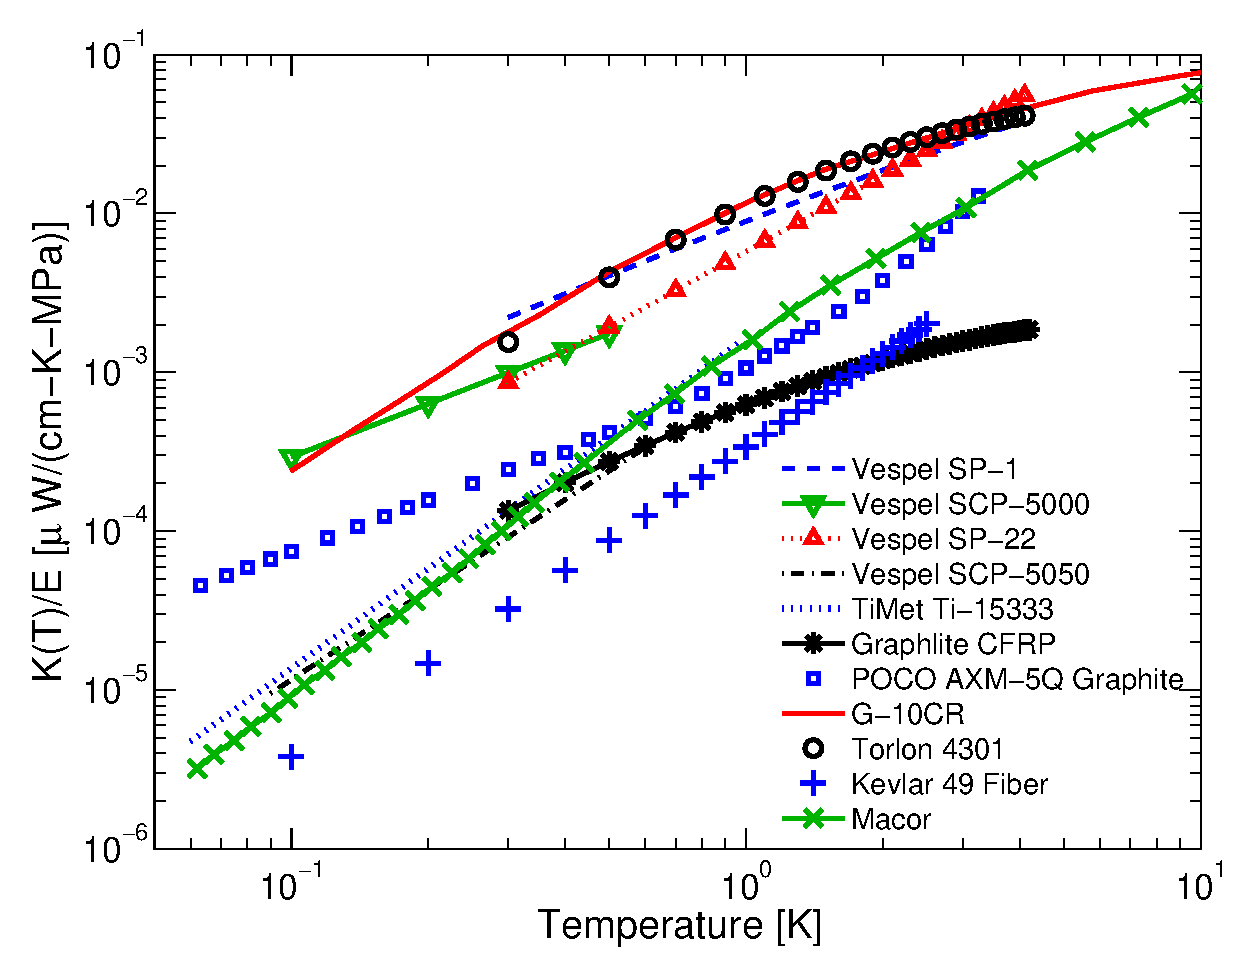
\includegraphics[%
  width=0.65\linewidth,
  keepaspectratio]{Mats}
\end{center}
\caption{A selection of popular and useful materials with their room temperature Youngs modulus normalized by their thermal conductivity.  Lower values correspond to materials with lower thermal conductivity to stiffness ratio, thus making them more ideal materials for support structures}
\label{Mats}
\end{figure}

\begin{figure}[!ht]
\begin{center}
\includegraphics[%
  width=0.65\linewidth,
  keepaspectratio]{SW}
\end{center}
\caption{Material properties of some select materials}
\label{SW}
\end{figure}

\section{Conclusions}
While many different solutions are available when creating cryogenic support structures, following certain design criteria and avoiding potential pitfalls that compromise structural strength allow for tube and truss structures to remain string while providing low heat loads between stages.  It is important to design with a large factor of safety beyond the theoretical failure point of a structure due to the imperfection dominated failure modes that exist in actual structures of this variety.  When considering truss members, tubes offer high stiffness but little to no elastic region before fracture.  Rods offer more elasticity which makes them susceptible to buckling.

\begin{acknowledgements}
We would like to thank S. Govindjee for technical assistance and use of his strength testing equipment. We acknowledge support and funding from the Department of Energy and the National Science Foundation.
\end{acknowledgements}

\begin{thebibliography}{99}

\bibitem{Hastings1993}
Peter R. Hastings and D.M. Montgomery. Support of cooled components in astronomical instruments. Cryogenics, 33(11):1032–1036, 1993.

%%%%%% Young's modulus bibliography items %%%%%%%%%
%%%%%%%%%%%%%%%%%%%%%%%%%%%%%%%%%%%%%%%%%%%%%%%%%%%

\bibitem{Doty1981}
F.D. Doty and P.D. Ellis, {\it Rev. Sci. Instrum.} \textbf{52(12)}, 1868, (1981).

\bibitem{Kasen1981}
M.B. Kasen, G.R. MacDonald, D.H. Beekman, Jr., and R.E. Schramm, {\it Advances in Cryogenic Engineering Materials} \textbf{26}, 235, (1981). 

%%%% Thermal conductivity bibliography items %%%%
%%%%%%%%%%%%%%%%%%%%%%%%%%%%%%%%%%%%%%%%%%%%%%%%%

%\cite{}

%%% Vespel SP-1, Vespel SP-22, Graphlite CFRP, Torlon 4301
\bibitem{Runyan2008}
M.C. Runyan and W.C. Jones, {\it Cryogenics} \textbf{48}, 448, (2008).

%%% Vespel SCP-5000, Vespel SCP-5050, Ti 15-3-3-3
\bibitem{Kellaris2013}
N.A. Kellaris. {\it Unpublished thermal conductivity measurements}, (2013).

%%% AXM-5Q
\bibitem{Woodcraft2009}
A.L. Woodcraft, M. Barucci, P.R. Hastings, L. Lolli, V. Martelli, L. Risegari, and G. Ventura, {\it Cryogenics} \textbf{49}, 159, (2009).

%%% G-10CR & Macor
\bibitem{Wood2009}
A.L. Woodcraft and A. Gray, {\it Low Temp. Detectors 13, Proceedings of the 13$^{th}$ International Workshop}, \textbf{1185}, 681, (2009).

%%% Kevlar 49
\bibitem{Ventura2009}
G. Ventura and V. Martelli, {\it Cryogenics} \textbf{49}, 376, (2009).

\end{thebibliography}

\end{document}
